% Template LaTeX file for DAFx'06 papers
%
% To generate the correct references using BibTeX, run
% latex, bibtex, latex, latex
% modified from DAFx-00 version by Florian Keiler, 2002-07-08
% from DAFx-02 to DAFx-03 by Gianpaolo Evangelista  
% from DAFx-04 to DAFx-05 by Javier Casajus  
% from DAFx-05 to DAFx06 by Vincent Verfaille

\documentclass[a4paper]{article}
\usepackage{dafx_06,amssymb,amsmath} 
\setcounter{page}{1}
\ninept

% pdf-tex settings:
% ------------------------
% detect automatically if run by latex or pdflatex
\newif\ifpdf  
\ifx\pdfoutput\undefined
   \pdffalse
\else
   \pdfoutput=1
   \pdftrue
\fi

\ifpdf % compiling with pdflatex
  \pdfcompresslevel=9
  \usepackage[pdftex]{graphicx}
\else % compiling with latex
  \usepackage[dvips]{graphicx}
\fi

\usepackage{times} 
  % saves a lot of ouptut space in PDF...
  % ..after conversion with the distiller         
  % Delete if you cannot get PS fonts working on your system.

\title{A New Paradigm for Sound Design}
% The following command replaces \name{The DAFx Crew} 
%%%%%%%%%%%%%%%%%%%%%%%%%%%%%%%%%%%%%%%%%%%%%%%%%%%%%%
\affiliation{Ananya Misra, Perry R. Cook$^{\dag}$, Ge Wang}
{Department of Computer Science ($^{\dag}$also Music)\\Princeton University, Princeton, USA \\ \texttt{\{amisra, prc, gewang\}@cs.princeton.edu}}

\begin{document}
% more pdf-tex settings:
% ------------------------
\ifpdf % used graphic file format for pdflatex
  \DeclareGraphicsExtensions{.png,.jpg}
\else  % used graphic file format for latex
  \DeclareGraphicsExtensions{.eps}
\fi
% ------------------------
\maketitle

\begin{abstract}
A sound scene can be defined as any ``environmental'' sound that has a
consistent background texture, with one or more potentially recurring
foreground events. We describe a data-driven framework for analyzing,
transforming, and synthesizing high-quality sound scenes, with flexible
control over the various components that make up the synthesized sound.
Given one or more sound scenes, we provide well-defined means to: (1)
identify points of interest in the sound and extract them into reusable
templates, (2) transform sound components independently of the background
or other events, (3) continually re-synthesize the background texture in a
perceptually convincing manner, and (4) controllably place event templates
over the background, varying key parameters such as density, periodicity,
relative loudness, and spatial positioning. Contributions include:
techniques and paradigms for template selection and extraction, independent
sound transformation and flexible re-synthesis; extensions to a
wavelet-based background analysis/synthesis; and user interfaces to
facilitate the various phases. Given this framework, it is possible to
completely transform an existing sound scene, dynamically generate sound
scenes of unlimited length, and construct new sound scenes by combining
elements from different sound scenes.
Url: http://taps.cs.princeton.edu
\end{abstract}

\section{Introduction}

Many sound synthesis techniques focus on generating foreground sounds, 
which by themselves do not generally give a listener 
a strong sense of being in a real-world environment. This paper introduces 
techniques and paradigms for working with the totality of foreground and background 
sounds that compose a sound scene.
%Existing methods that deal with pre-recorded sound do not 
%provide suitable analysis and synthesis techniques for truly flexible ``sound 
%scene modeling by example,'' where a sound scene can be composed from selected 
%components of different example sounds. 
%The goal is to enable the creation of perceptually convincing 
%sound scenes from a set of existing sounds, with the generated sound  
%being arbitrarily close to or different from the original sounds, based on 
%the user's intention. 
Existing methods that deal with pre-recorded sound do not 
provide suitable analysis and synthesis techniques for a sound scene to be composed 
from selected components of different existing sounds.
Naive approaches such as repeatedly playing or combining 
raw segments of original recordings do not sound convincing, while more complex 
synthesis methods lack flexibility both in creating scenes and in the 
amount of user control needed.
%The generated sound should be arbitrarily close to or different from the 
%original, so that it can either be perceived as another instance of it or 
%as a completely different scene. Since repeatedly playing the original 
%sound is not convincing, the synthesis should involve some randomness as 
%well as a flexible amount of user control. NOT MAKING SENSE AS A PARAGRAPH.

Given one or more existing sound scenes, our task is to generate from 
these any amount of perceptually convincing sound, arbitrarily similar to 
or different from the original sounds, that can be parametrically controlled to fit the user's 
specifications. One of our aims is to provide a flexible tool for 
easily modeling and generating sound scenes for 
entertainment (movies, TV, and games), Virtual and Augmented Reality, 
and art projects such as live performances and installations.
Towards this aim, we introduce TAPESTREA: Techniques and Paradigms for 
Expressive Synthesis, Transformation and Rendering of Environmental 
Audio. Our approach is based on the notion that sound scenes are 
composed of events and background sound, which are best modeled 
separately. We separate a sound scene into the following 
components:
(1) \emph{Deterministic events}: composed of highly sinusoidal components, 
often perceived as pitched events, such as a bird's chirp or a baby's cry;
(2) \emph{Transient events}: brief non-sinusoidal events, such as footsteps;
(3) \emph{Stochastic background}: the ``din'' or residue remaining after the 
removal of deterministic and transient components, such as wind, ocean waves, or 
street noise.

%TAPESTREA analyzes and synthesizes each component separately. It  
%applies spectral modeling \cite{Serra89} to extract deterministic events 
%and a stochastic residue from a given sound. The deterministic events are 
%then generated to order, possibly after spectral transformations, using 
%sinusoidal re-synthesis. TAPESTREA isolates and extracts transients either before or 
%after the spectral modeling analysis. The final stochastic background is 
%obtained by removing the deterministic as well as transient events 
%from the given sound and filling in the holes left by transient removal. 
%Once the background component has been separated, the system dynamically 
%generates it using a wavelet tree learning algorithm by Dubnov et. al. 
%\cite{Dubnov02}, with significant improvements. Running this algorithm 
%on a stochastic background with no sinusoidal components allows the wavelet 
%tree learning to operate on the type of data with which it works best.  

TAPESTREA analyzes and synthesizes each component separately, using algorithms suitable 
to the component type. It applies spectral modeling \cite{Serra89} to extract deterministic 
events, and time-domain analysis to detect transient events. Each event can then be 
transformed and synthesized individually. The stochastic background is obtained by 
removing deterministic and transient events from the given sound and filling in the 
holes left by transient removal; background is then dynamically generated using an improved wavelet 
tree learning algorithm \cite{Dubnov02}.

TAPESTREA is distinct from other sound analysis and synthesis methods in that it allows users to:
(1) point at a sound or a part of a sound, extract it, and request more or less of it in the final scene,
(2) transform that sound independently of the background,
(3) flexibly control important parameters of the synthesis, such as density, periodicity, relative gain, and spatial positioning of the components
(4) construct novel sounds in a well-defined manner.

%  Put this somewhere else maybe:  SMS techniques has been primarily used for 
%  analysis/modeling of foreground musical sounds.  We are the first (and the last probably) to 
%  use it for event separation in texture synthesis.

%Our method also allows users to have control over the characteristics of their synthesized 
%texture. Separating the events provides a framework in which to manipulate events 
%individually, and to request more occurences of some events and less of others in the final 
%texture. It also offers the option or creating new sound textures by mixing the backgrounds 
%and deterministic events from several example textures.

%PLACEHOLDER: our contributions are too numerous to list here, a random sampling:
% observation: separation of foreground events and background din is beneficial
%    - indepedently transform events and background
%    - you can add or remove instances of events
%    - mix events from different sources
%    - better results (we hope) from wavelet
% contribution:
%    - system for doing it
%    - a user interface for building new sound textures

%   1.1 Motivation\\
%   		 - what is a sound texture anyway?\\
%       - "i have this sound texture, I want to produce more of it.
%          and in this way (clarifify)"\\
%       - give sound designers automation tool\\
%   1.2 Our general approach (what we are describing in this paper)\\
%	- we like wavelet tree learning and we like sms\\
%	- we want to realize the future section of wavelet tree, be able to point at 
%components of a sound and ask for more or less of it\\
%	- using sms plus feature based audio classification we gain\\
%	---we can separate out events/foreground\\
%	---we make wavelet tree better because we separate harmonic events, which wavelet tree 
%is not good at handling\\
%	- transform: because we have individual events we can modify and place them 
%independently\\
%	- more control over the textures we synthesize (example somewhere)\\

%CONTRIBUTIONs listed above (not commented out)

The rest of the paper is structured as follows: In Section 2 we describe 
related work. Section 3 provides an overview of our 
approach along with an example highlighting how it can be used. Section 4 
describes the analysis stage of our framework, section 5 describes the possible 
transformations on events, and section 6 describes the synthesis phase. 
Section 7 provides details about our user interface and section 8 summarizes results 
and contributions. Section 9 describes our conclusions and directions for future work. 


\section{Related Work}

%Previous work on synthesizing sound to match a given environment has 
%involved simulation or model-based methods for generating interactive 
%contact sounds, or the analysis and re-synthesis of existing sounds. 
%Tools for sound production also include a range of sound editors. 

%Related work includes the following methods for sound analysis and synthesis, 
%and tools for sound production.

\subsection{Simulated and Model-based Foreground Sounds}

Simulation and model-based sound synthesis techniques are based on physical models of the 
objects, the world, and/or the interactions between these \cite{CookBook}. 
Physically based models have been used to generate foreground sounds  
caused by object interactions, including walking sounds \cite{Cook02}, sounds caused by the motion of 
solid objects \cite{OBrien01}, complex sounds due to individual objects and gestures 
\cite{Rocchesso03}, and contact sounds \cite{Doel01} such as colliding, rolling, and 
sliding. 

%Aerodynamic sounds \cite{Dobashi03} have been rendered using computational fluid dynamics. 
%Models of a virtual environment have also been used for effective sound 
%rendering \cite{Takala92,Tsingos04}.

%Physics based motion-driven synthesis \cite{Cardle03, Dobashi03}.

%The advantage of simulated and model-based approaches is that given a model, sound can be
%directly inferred, synthesized, and transformed by modifying the model parameters. 
%However, the requirement of having a model in order to generate sound  makes these methods 
%difficult to generalize. Production audio often uses pre-recorded sounds instead of models; it is 
%therefore worthwhile to make the processing of pre-recorded sounds as parametric as possible. 

%this is not what we are doing.

\subsection{Background Sound Textures}
%\subsection{Sound Textures}

A sound texture can be described as a sound with structural elements 
that repeat over time, but with some randomness. The sound of rain falling 
or applause are examples of sound textures. 
Textures often form a large part of the background of sound scenes.

Athineos and Ellis \cite{Athineos03} modeled sound textures composed of
very brief granular events known as \textit{micro-transients}, such as 
fire crackling or soda being poured out of a bottle. 
Zhu and Wyse \cite{Zhu04} extended their technique to separate 
the foreground transient sequence from the background din in the source 
texture and resynthesized these separately. Both these methods are effective on textures 
that primarily contain micro-transients, but do not generalize well to other sounds. For 
instance, the foreground-background separation misses spectral foreground events, as it does 
not take frequency into account while identifying events.

Miner and Caudell \cite{Miner97} used wavelets to decompose, 
modify, and re-synthesize sound textures, concentrating 
on the perceptual effects of various transformations. 
Dubnov et. al. \cite{Dubnov02} also used a wavelet decomposition to 
analyze and generate more of a sound texture. 
Their method works well for sounds that are mostly 
stochastic or have very brief pitched portions. However, sounds with 
continuous components, such as a formula-one racecar engine, sometimes 
get chopped up, while rhythmic sounds may lose their rhythm during 
synthesis. The stochastic model is also not suitable for sounds with 
many sinusoidal components.
 
In general, these existing approaches work only for mostly stochastic sounds and 
do not allow flexible control over the output---either the entire texture is 
transformed or segments are shuffled and concatenated. Hence 
these methods are insufficient for sounds that have various foreground events and 
background playing simultaneously.
Our approach overcomes these limitations by isolating and removing 
pitched sounds, performing modified wavelet tree learning 
\cite{Dubnov02} on the  
remaining stochastic part, and re-inserting the extracted components 
afterwards. We separate the pitched components from the sound texture 
using spectral modeling.

%Given an existing ambient/background/environment sound of limited, 
%length, it is possible to synthesize more of the same texture. This 
%method has no prior knowledge of the objects in the environment. 


%       - texture synthesis from existing ambient/background/environment
%         sounds (of limited length)\\
%       - LPC fails (probably)\\
%         --- good for micro-transients\\
%       - dubnov et. al.  (2002)\\
%         --- showed how to take apart and synthesize more of it but...\\
%         --- individual events not good for chopping up, not good for repeating\\
%       - miner and caudell\\
%       - we come in here...\\
%         --- event identification/isolation/transformation/(authentification)
%           (better analysis)\\
%         --- take better advantage of wavelet tree learning \\
%         --- separation of control over background and events
%           (more control during synthesis)\\
%         --- more potential for interactivity\\
%         --- combine many of these approachs + spectral modeling\\
%         --- talk about how our stuff differs\\

\subsection{Spectral Modeling}

Spectral modeling \cite{Serra89} extends the original sinusoidal modeling algorithm 
\cite{McAulay86} by posing the concept of ``sines plus noise,'' based on the notion that 
some components of sound fit a sinusoidal model while others are better modeled by spectrally 
shaped noise. While Serra and Smith \cite{Serra89} initially applied this to musical instrument 
sounds, we use it to extract \emph{deterministic events} from any recorded sound scene. 
Sinuosoidal modeling also enables modification of the original sound before re-synthesis, for
instance by pitch-shifting and time-stretching.
Other related work on spectral analysis includes alternatives to 
the Fourier transform for estimating the spectra of specific kinds of 
signals \cite{Qi02,Thornburg03}. 

Existing tools for spectral analysis and re-synthesis, such as SPEAR \cite{Klingbeil05}
and the CLAM library \cite{Amatriain05}, allow high-level sinusoidal analysis, 
transformations and re-synthesis, but do not offer the level of parametric control over 
these stages suitable for analyzing and creating sound scenes. Further, they lack a 
framework for processing transients and stochastic background components.

\subsection{Sound Editors}

Current tools for commercial or home audio production include a range of sound editors. Free 
or inexpensive commercially available software such as Audacity and GoldWave perform simple 
audio production tasks. Midline audio editing systems, including Peak, Logic, and Cubase, are 
geared towards music production and often offer real-time MIDI sequencing capability. At the 
high end are digital audio production hardware/software systems such as Pro Tools, geared 
towards commercial sound production. Most of these products support Virtual Studio Technology 
(VST) plug-ins that perform synthesis algorithms and apply effects such as reverb. However, 
none of them provides one real-time, extensible, integrated analysis-transformation-synthesis 
workspace.  

%\begin{equation}
% \sum_{j=1}^{z} j = \frac{z(z+1)}{2}
%\end{equation}

\section{Example and Overview of our Approach}

The TAPESTREA system starts by loading a 5--15 seconds or longer existing sound scene, 
such as the sound of a city street, seagulls by the ocean or children playing in a park. 
Sound events in the park scene may include children yelling,  
a ball bouncing, and geese honking in a nearby pond. The background texture might 
consist of the general din of the surroundings. 
%No {\it a priori} knowledge of the existing sound is needed; users can interactively 
%direct its operation for specific results.  

\begin{figure}[t]
\centering
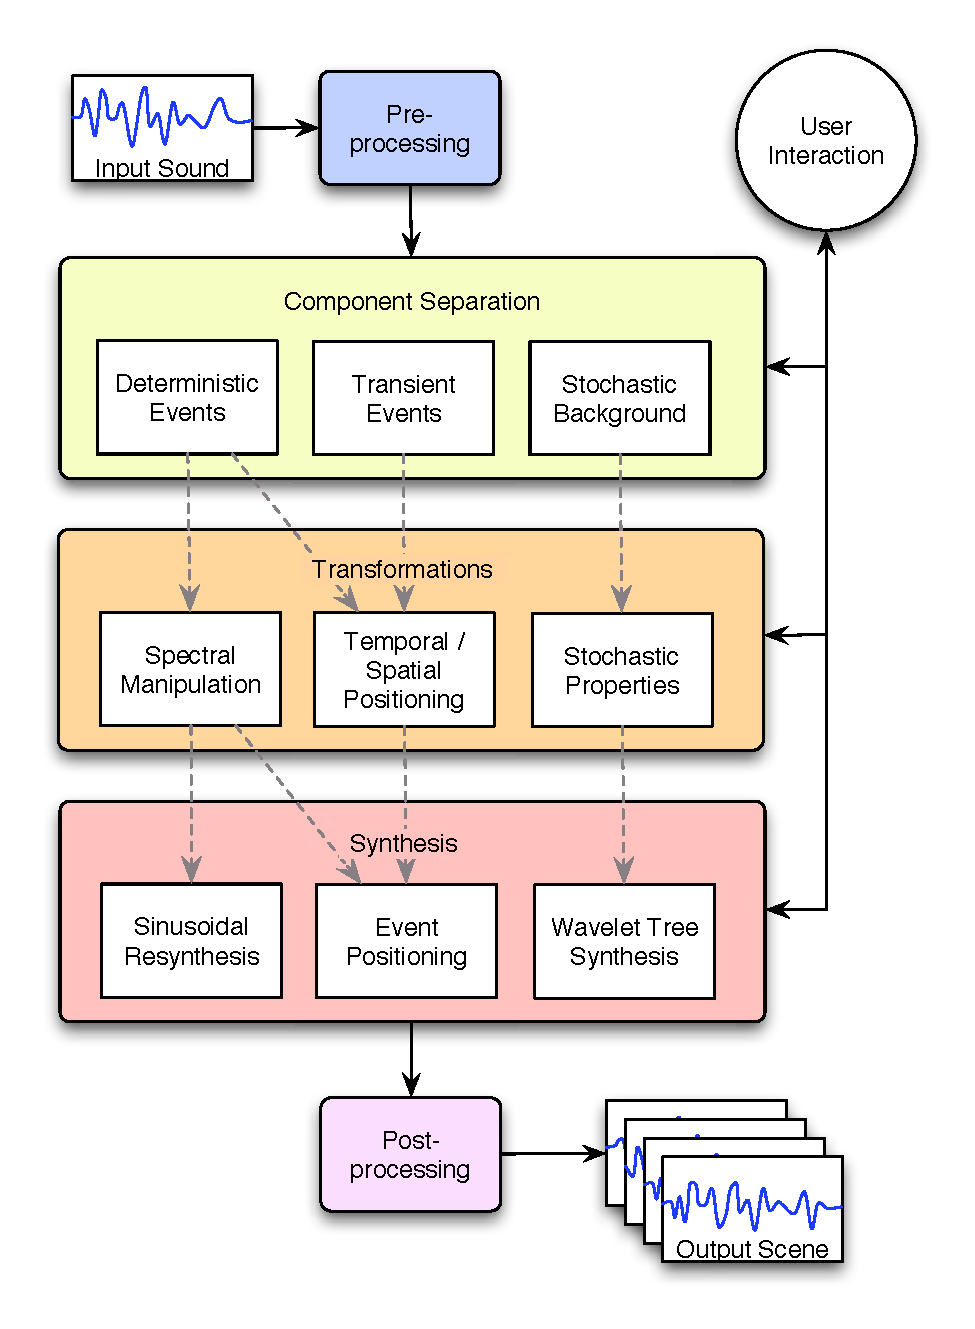
\includegraphics[width=.93\columnwidth]{ourpipeline2.eps}
\caption{Stages in our pipeline: (1) preprocessing, (2) analysis, (3) transformation, (4) synthesis}
%The preprocessed sound is analyzed to enable component separation. These components undergo optional transformations before they are individually synthesized and combined to produce the final sound.}
\label{fig:pipeline}
\end{figure}

Figure \ref{fig:pipeline} depicts the phases in the TAPESTREA pipeline. The existing sound scene first
undergoes a basic preprocessing phase involving sample-rate/data-depth 
conversion as needed, channel information, DC blocking and data normalization. Next, it passes through the 
analysis phase, where the user extracts deterministic (children yelling, geese honking), 
transient (ball bouncing) and stochastic background (general din) 
components by specifying analysis parameters. Each component can be played back separately 
and stored as a template for future use. For example, one bounce of the ball can 
be stored as a transient template while individual yells can be saved as deterministic event 
templates. In the transformation and synthesis phase, the system or user parametrically specifies 
how to construct the output sound scene. Transformations are applied to individual 
templates and these templates are combined in specified ways to generate a complete sound scene. 
For instance, the output sound scene can consist of a repeatedly bouncing ball and many children yelling 
at different pitches and times over a continuous general din, to simulate a 
children's game with enthusiastic spectators in a park without geese. The output sound can also 
include templates from other existing sound scenes, such as a referee's whistle. The synthesized 
sound scene can be written to a file or played continuously in real-time 
for as long as needed. TAPESTREA also includes a graphical user interface for interactive control 
of the analysis, transformation and synthesis parameters. The following sections provide more in-depth 
information on the processing phases and the user interface. 

\section{Event Identification and Isolation}

The first step in our framework is to identify and separate foreground events from 
background noise. Foreground events are parts of the scene perceived as distinct occurrences, and 
include both \emph{deterministic events} (the 
sinusoidal or pitched components of a sound) and \emph{transient events} (brief bursts 
of stochastic energy). Removing these leaves us with the \emph{stochastic background}. 

%\subsection{Preprocessing}

%We are considering several ways of preprocessing the given sound 
%texture to enhance deterministic and transient event extraction. One strategy is to bandpass-filter 
%the sound and perform event detection separately on each subband. This 
%could be useful because what is perceived as an event may differ according 
%to the spectral range in which it takes place. For example, high-frequency
%sounds
%(specific range?)
%are easier to detect than low-frequency sounds of 
%the same magnitude (I think). So processing each subband separately allows 
%for better fine-tuning of the event detection / tracking parameters.
%
%Another form of preprocessing is to intelligently segment the given sound 
%texture using the MARSYAS framework. Each segment could then be processed 
%separately. Since each segment is a contiguous-time clip with uniform 
%features, doing this could also aid event identification.
%
%The thing we actually do is block DC.
%
%\subsection{Classification}
%
%PROBABLY DITCH CLASSIFICATION, AND LEAVE IT FOR FUTURE WORK.
%As described earlier, classification of 
%sounds can give us hints on the appropriate parameters or techniques to use for event detection and 
%tracking. We can classify based on various features, including power, spectral centroid and 
%rollof, spectral flux, zero crossing rate, and Mel-Frequency Cepstral Coefficients. For 
%domain-specific tasks, features such as Parametric Pitch Histogram, and Beat/Periodicity 
%Histogram can be calculated and used. These features also aid segmentation of the original 
%sound, as described in Section 4.1.

\subsection{Sinusoidal Modeling}

Deterministic events are identified through sinusoidal analysis based on the 
spectral modeling framework. The input sound scene is read in as possibly overlapping 
frames, each of which is transformed into the frequency domain using the 
FFT and processed separately. The maximum and average 
magnitudes of the spectral frame are computed and stored. The following 
steps are then repeated until either a specified maximum number (N) of peaks 
have been located or no more peaks are present:
%The lowest frequencies in the spectral frame are eliminated to avoid 
%artifacts from the transform and windowing.
%(kind of ambiguous)(why?)
(1) The maximum-magnitude bin in the frame, within the specified frequency range, is 
located. 
(2) If the ratio of its magnitude to the average magnitude of the frame is 
below a specified threshold, it is assumed to be noise and we deduce that no 
more peaks are present. 
(3) If its magnitude is above a specified absolute threshold, it is added as a 
sinusoidal peak and the bins it covered are zeroed out in the analysis frame.
\begin{figure}[t]
\setlength\textfloatsep{0pt}
\setlength\abovecaptionskip{0pt}
\setlength\belowcaptionskip{0pt}
\centering
   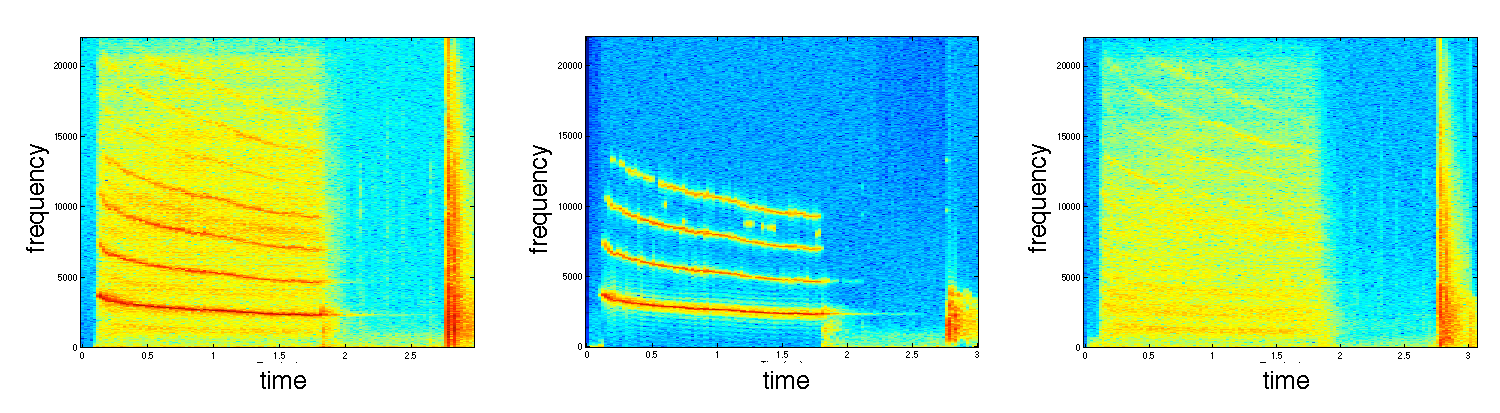
\includegraphics[width=.48\textwidth]{fireworks3.eps}
%  \subfigure[]{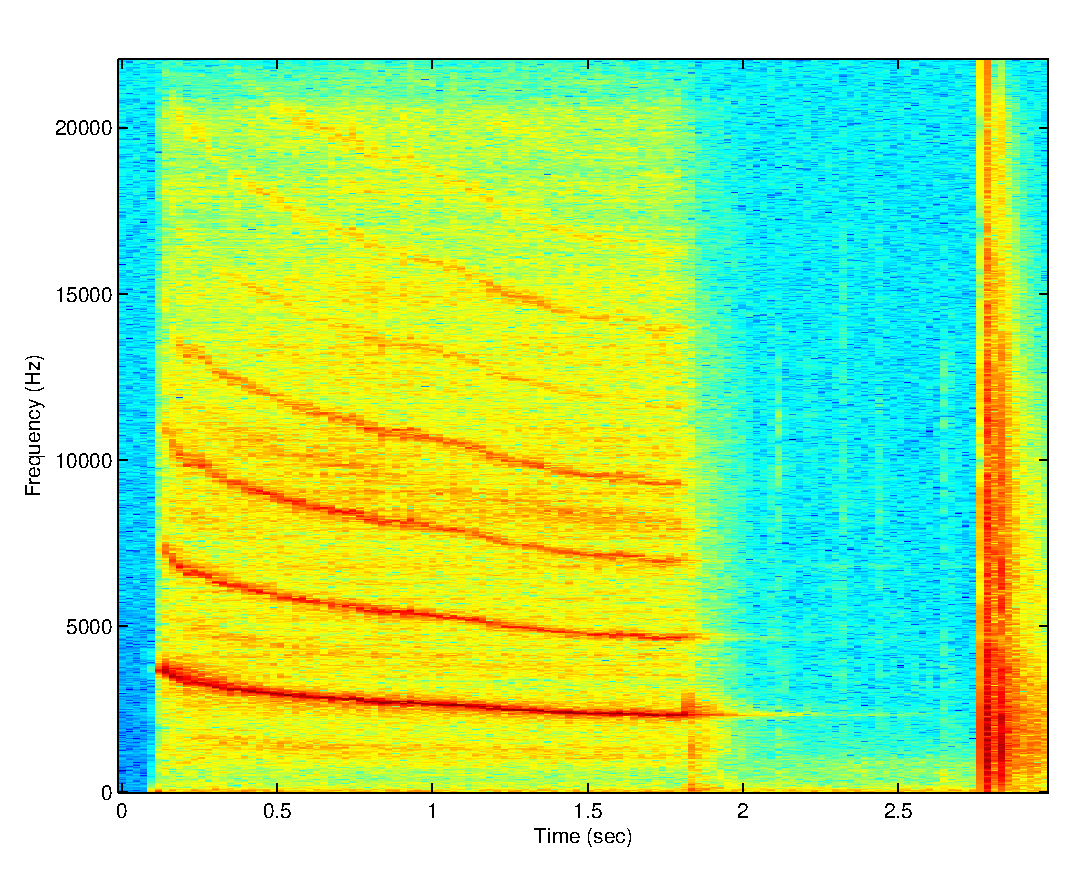
\includegraphics[width=.155\textwidth]{firework.eps}}
%  \subfigure[]{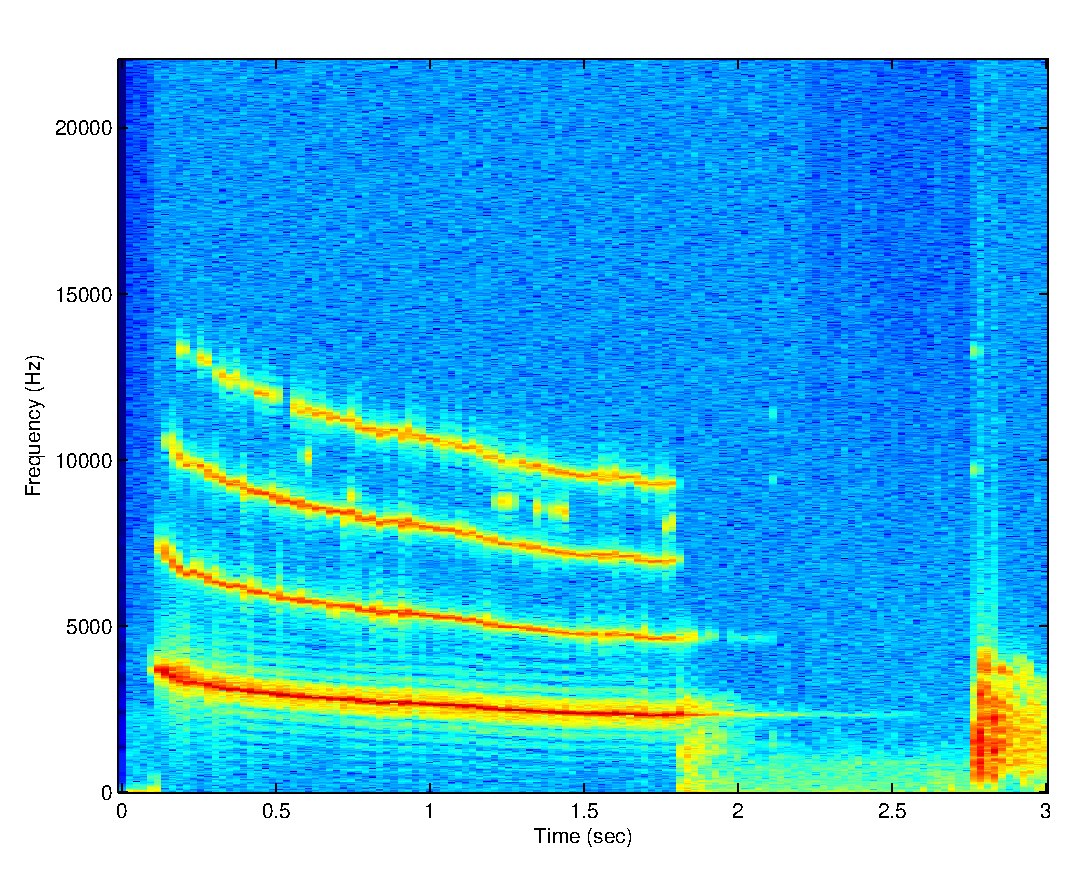
\includegraphics[width=.155\textwidth]{fireworktracks2.eps}} %.7159*.22=.1575
%  \subfigure[]{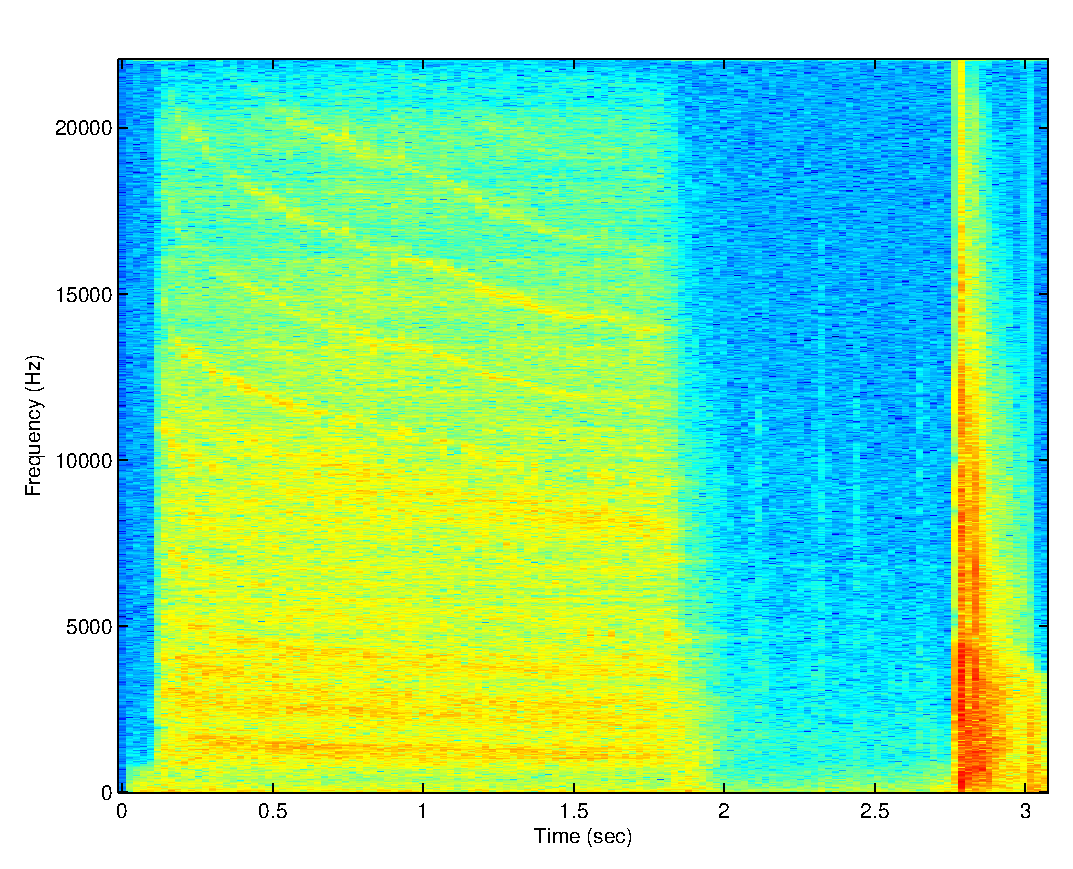
\includegraphics[width=.155\textwidth]{fireworkres2.eps}}
\caption{Separating sinusoidal tracks from stochastic residue: (a) original sound; 
(b) sinusoidal tracks; (c) residue}
\label{fig:sines}
\end{figure}

All the sinusoidal peaks and FFT frames can also be precomputed and stored. 
All peaks in a frame are found by locating bins where the derivative of the magnitude changes from 
positive to negative. The peaks for each frame are stored in decreasing magnitude order.
At run-time, the top N peaks that satisfy any frequency and threshold 
bounds are selected per frame for peak matching. 

Once the top N peaks in all the frames have been collected, peaks are matched  
from frame to frame if they occur at sufficiently similar frequencies. 
Over time this yields \emph{tracks} of peaks lasting across frames. The 
matching and updating of tracks takes place as follows:
(1) Each existing track from previous frames selects a current frame peak 
closest to it in frequency. If the difference in 
frequency is above a specified threshold, that track is dormant 
and the selected peak remains unmatched. 
(2) All unmatched peaks are 
added as new tracks, and all existing tracks that have not found a 
continuation are removed if they have remained dormant for a specified 
number of frames. 
(3) Tracks that continue across a specified minimum number of frames are retained. 

Finally, TAPESTREA can parametrically group related tracks \cite{Ellis94,Melih00} 
to identify events. A track is judged to belong in an existing group if it has a 
minimum specified time-overlap with the group and either: (1) its frequency is harmonically 
related to that of a track in the group, (2) its frequency and amplitude 
change proportionally to the group's average frequency and amplitude, 
or (3) it shares common onset and offset times with the group average. If a track 
fits in multiple groups, these groups are merged. While the grouping could 
benefit from a more sophisticated algorithm or machine learning, it may be 
fine-tuned for specific sounds by manipulating error thresholds for each grouping 
category. Groups that last over a specified minimum time span are considered 
deterministic events. If grouping is not selected, all 
the tracks found are together considered a single event. Each deterministic 
event is defined a list of sinusoidal tracks, with 
a history of each track's frequency, phase and magnitude, and onset and completion times. 

The residue, or the sound with deterministic components removed, is extracted 
after the sinusoidal tracks have been identified. TAPESTREA eliminates 
peaks in a sinusoidal track from the corresponding 
spectral frame by smoothing down the magnitudes of the bins beneath the peak. 
It also randomizes the phase in these bins. Figure ~\ref{fig:sines} shows sinusoidal 
separation results. 

\subsection{Transient Detection and Separation}

Transients are brief stochastic sounds with high energy. While a sinusoidal track 
looks like a near-horizontal line on a spectrogram, a transient 
appears as a vertical line, representing the simultaneous presence of information 
at many frequencies. Transients are usually detected in the time domain by observing 
changes in signal energy over time \cite{Verma98,Bello05}. 
TAPESTREA processes the entire sound
using a non-linear one-pole envelope follower filter with a sharp attack and gradual 
decay to detect sudden increases in energy. Points where the ratio of the envelope's derivative 
to the average frame energy is above a user-specified threshold mark transient onsets. A transient's length  
is also user-specified and can thus include any amount of the decay. Other real-time analysis parameters 
include the filter attack and decay coefficients, and aging amount in computing average frame energy.
Transient events, being brief and noisy, are represented as raw sound clips, although they can also be modeled 
by peak picking in the time domain \cite{Verma98}.
%Transient events are not well represented by sinusoidal tracks as they 
%contain many different frequencies, but can be modeled by peak picking in the 
%time domain \cite{Verma98}. However, they are generally brief and continuous enough to be 
%stored as raw sound clips; this is how we represent them. 

Detected transients are removed, and the resulting ``holes'' are filled by applying 
wavelet tree resynthesis \cite{Dubnov02}. 
The nearest transient-free segments before and after a transient event are 
combined to estimate the background that should replace it. Wavelet tree 
learning generates more of this background, which is overlap-added into the original 
sound to replace the transient. The residue from the sinusoidal analysis, with transients 
removed in this way, is saved to file and used for stochastic background generation in the 
synthesis phase. Figure ~\ref{fig:transient} demonstrates the hole-filling. 
\begin{figure}[t]
\setlength\textfloatsep{0pt}
\setlength\abovecaptionskip{0pt}
\setlength\belowcaptionskip{0pt}
\centering
   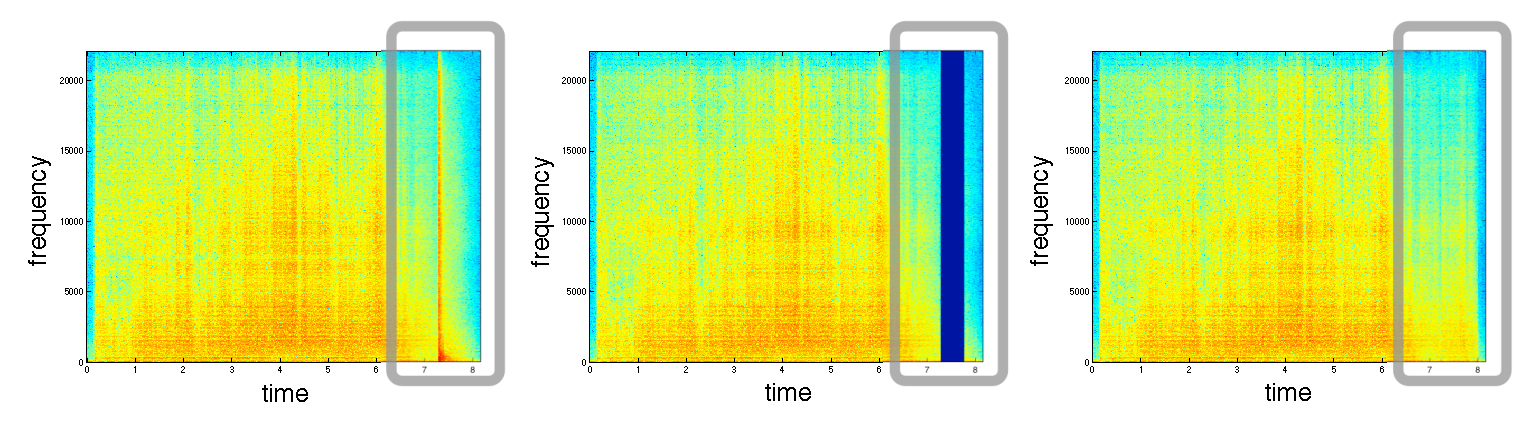
\includegraphics[width=.48\textwidth]{transient3.eps}
%  \subfigure[]{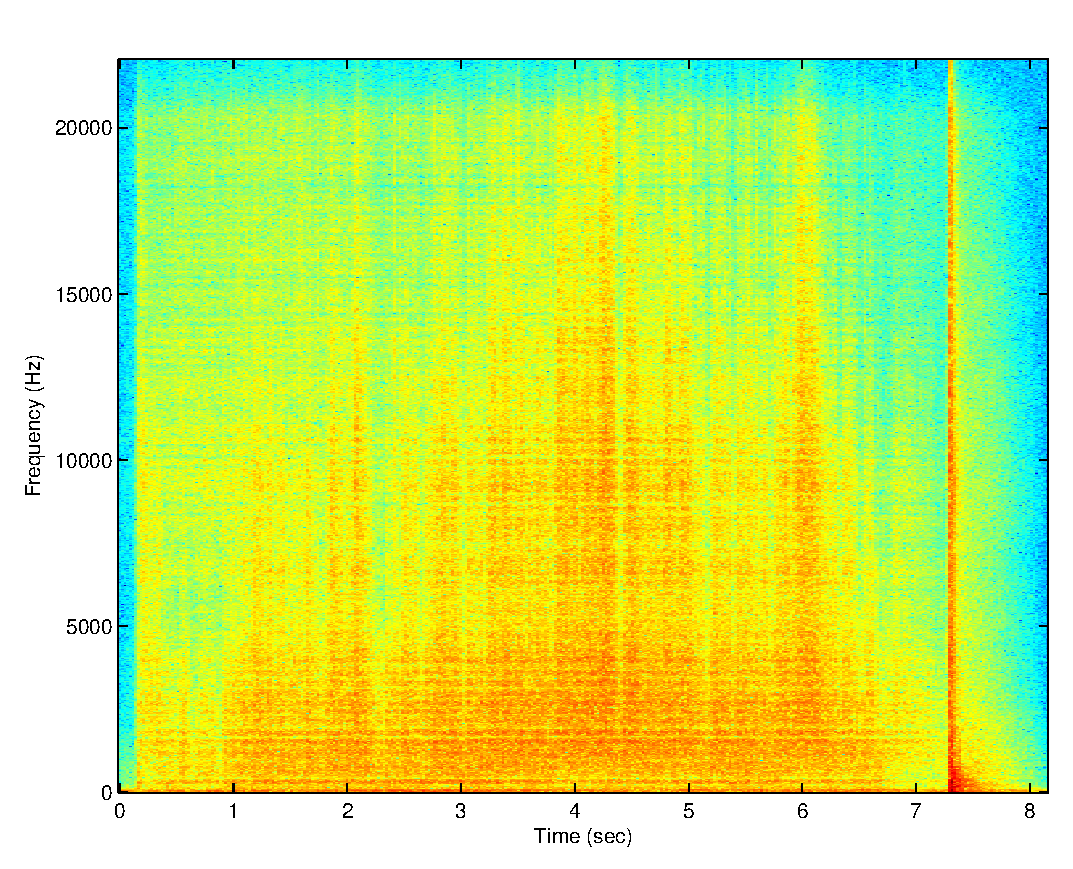
\includegraphics[width=.155\textwidth]{transient.eps}}
%  \subfigure[]{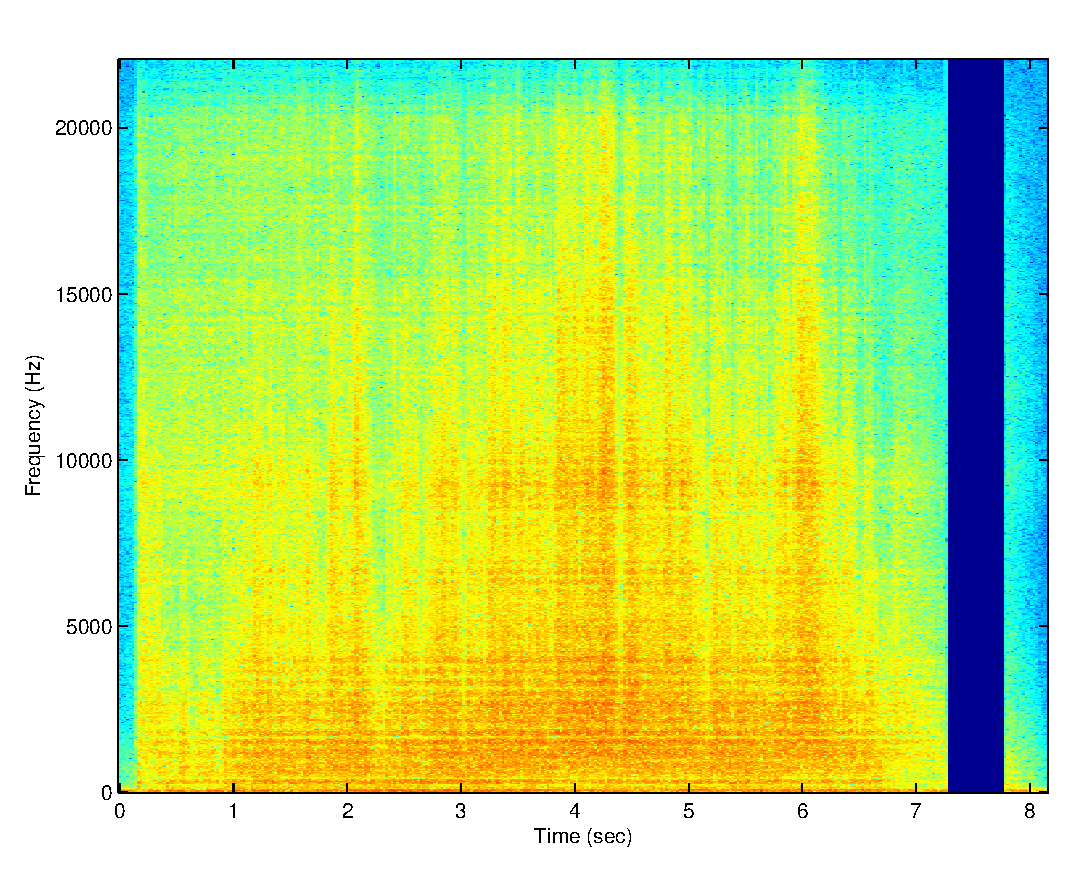
\includegraphics[width=.155\textwidth]{transient-.eps}}
%  \subfigure[]{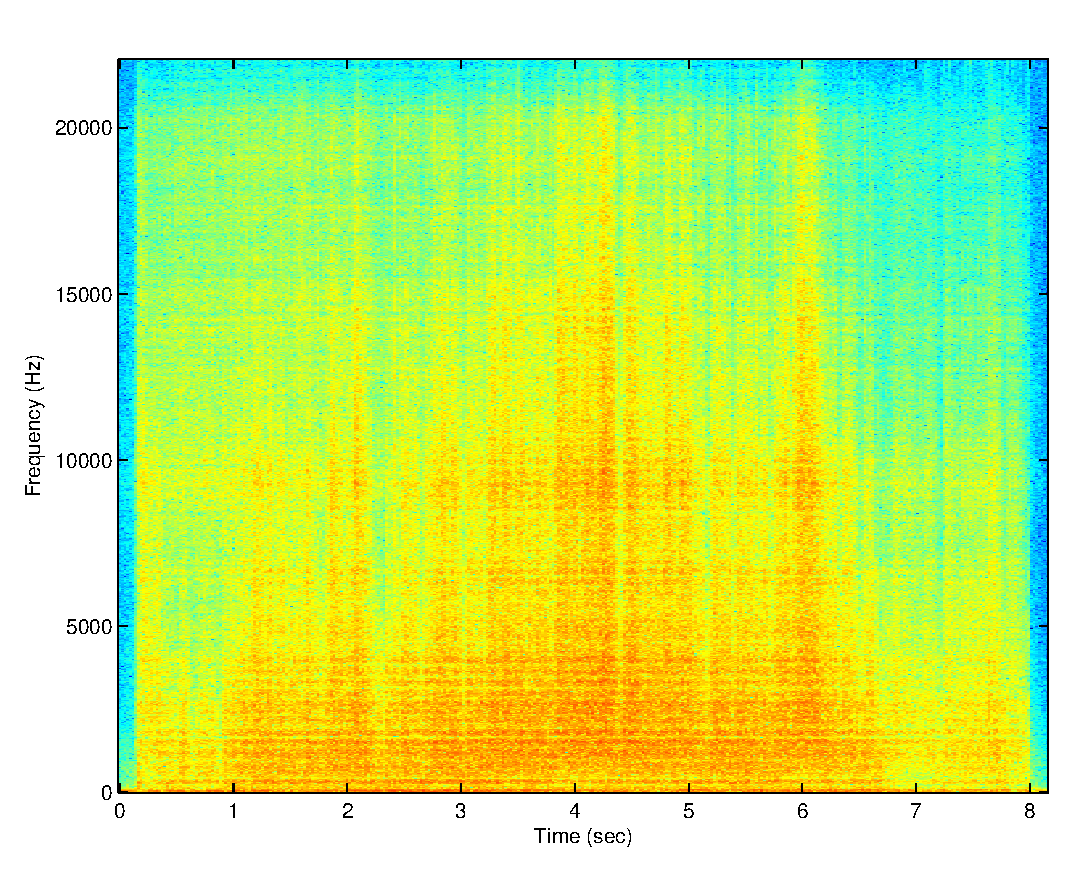
\includegraphics[width=.155\textwidth]{transient+.eps}}
\caption{Transient removal and hole filling: (a) fireworks with pop (at 7.2 sec); (b) 
fireworks with pop removed; (c) fireworks with hole filled}
\label{fig:transient}
\end{figure}
\section{Transformations}

We now have \emph{deterministic events} isolated in time and frequency from 
the background, \emph{transient events}, and \emph{stochastic background} texture. 
Output sound scenes are parametrically constructed from these templates. The parametric model lets 
each transformation be applied to each component independently of others.

\subsection{Event Transformations}

By stretching or compressing spectral
data, we can raise or lower the \textbf{frequency} content of a sound without 
affecting its duration.  For deterministic events with sinusoidal tracks, 
TAPESTREA linearly scales the frequency at each point in each track, 
giving high fidelity frequency warping for almost any factor (limited by our 
range of hearing). For transients, it uses a standard phase vocoder \cite{Dolson86} to 
similarly scale the frequency for each frame.  

The track-based representation of deterministic events allows us 
to robustly change the \textbf{duration} of each track by almost any factor without 
producing artifacts, by scaling the time values in the time-to-frequency trajectories of their tracks. 
Both time-stretching and frequency-warping can take place in 
real-time for deterministic events. Time-stretching for transients once again uses a phase 
vocoder to stretch or shorten the temporal overlap between frames.  

TAPESTREA offers control over the \textbf{temporal placement} of an individual event, either explicitly or using 
a probability distribution for repeating events.  
Explicitly, an event instance can be placed on a timeline at a specified onset time. The timeline 
may also include other event instances and background sound. Repeating events can be defined by a mean 
event density and desired repetition periodicity, and generated according to these parameters by a Gaussian or other 
distribution.

\subsection{Stochastic Background Transformations}

It is possible to interactively control the similarity between an extracted background 
and the synthesized background generated from its template.
The similarity or randomness is governed by the wavelet 
tree learning (Section 6.2) parameters. Also, the generated background 
can play for any arbitrary amount of time.

\section{Synthesis}

TAPESTREA synthesizes a sound scene following the specified transformations. The background 
component and the events are synthesized separately and combined to produce the 
final scene. Each component can also be heard in isolation so that a user can determine its 
role in the final scene. Although we discuss transformation and synthesis in separate sections for 
clarity, these two aspects are closely related. For example, components can be 
transformed in certain ways even while they are being synthesized. 

\subsection{Event Synthesis}

Deterministic events are synthesized from their defining tracks with 
sinusoidal re-synthesis. The system linearly interpolates frequency and magnitude 
between consecutive frames before computing the time-domain sound from 
these. Transient events are directly played back or, if a frequency-warping or time-stretching 
factor is specified, analyzed and synthesized through a phase vocoder.

\subsection{Stochastic Background Generation}

The background is generated using an extension of the wavelet tree learning 
algorithm by Dubnov et. al. \cite{Dubnov02}. The extracted 
stochastic background is decomposed into a wavelet tree (Daubechies, 5 vanishing moments),  
where each node represents a wavelet coefficient. 
A new wavelet tree is learned, with nodes selected from the original tree 
by their context, within a specified randomness range.

We added the option of incorporating randomness into the first step of the 
learning, and modified the amount of context used (`k') to depend on 
the node's depth. We also found 
that we can avoid learning the coefficients at the highest resolutions, 
without perceptually altering the results. Since the wavelet tree is binary, learning 
at the highest levels takes longer, but randomizes mainly high-frequency information. 
The optimization let us build a real-time version of wavelet tree learning, 
with interactive control over the learning parameters. The wavelet tree learning also works 
better with the separated stochastic background as input since the harmonic events 
it would otherwise garble have been removed. 

\subsection{Putting It All Together}

To construct a sound scene, extracted background and events are combined 
to the user's preference. A scene of a specified length 
can be generated by placing templates on a timeline of the desired length. 
Infinitely long sound scenes can also be generated and modified on-the-fly. 
The improved wavelet tree algorithm sythesizes unlimited background texture, while 
event templates can be temporally placed against the background either with fine 
control or in an automated manner (see Section 5.1). 

This framework adapts to many techniques for synthesizing the final sound. A user may 
craft a sound scene by listening to and adjusting the components separately, based on how they 
sound as a group or individually. The combined sound can then be similarly sculpted. On the other 
hand, the synthesis can also be driven from a game or animation algorithm that specifies 
transformations according to parameters drawn from the game or animation itself.

\section{User Interface}

The user interface (Figure \ref{fig:ui}) is separated into two phases: analysis and 
synthesis. In the analysis stage, the user can load a sound file and view its waveform, 
frame-by-frame spectrum and spectrogram. These views allow the user to visually 
identify events and perform analysis on appropriate time and frequency regions to 
extract specific events. Time and frequency 
bounds for the analysis can be specified by adjusting range sliders in the waveform 
and spectrum views or by selecting a rectangle in the spectrogram view. The frame-by-frame 
spectrum also shows the sinusoidal analysis threshold. Direct 
control over many other analysis parameters (Section 4) is also available. 
Having adjusted the analysis parameters, the user starts analysis by clicking a button. 
The extracted events are then played separately, along with a frame-by-frame view of 
their spectrum (for deterministic events) or a zoomed in view of their 
waveform (for transient events). The stochastic background is similarly 
played and viewed, or loaded for further analysis. An 
extracted event or background can be saved as a template for use in 
the synthesis phase. The user may then perform further analysis on the same source sound or 
a different one, or move on to the synthesis phase.

\begin{figure}[t]
%\begin{figure*}[h]
\centering
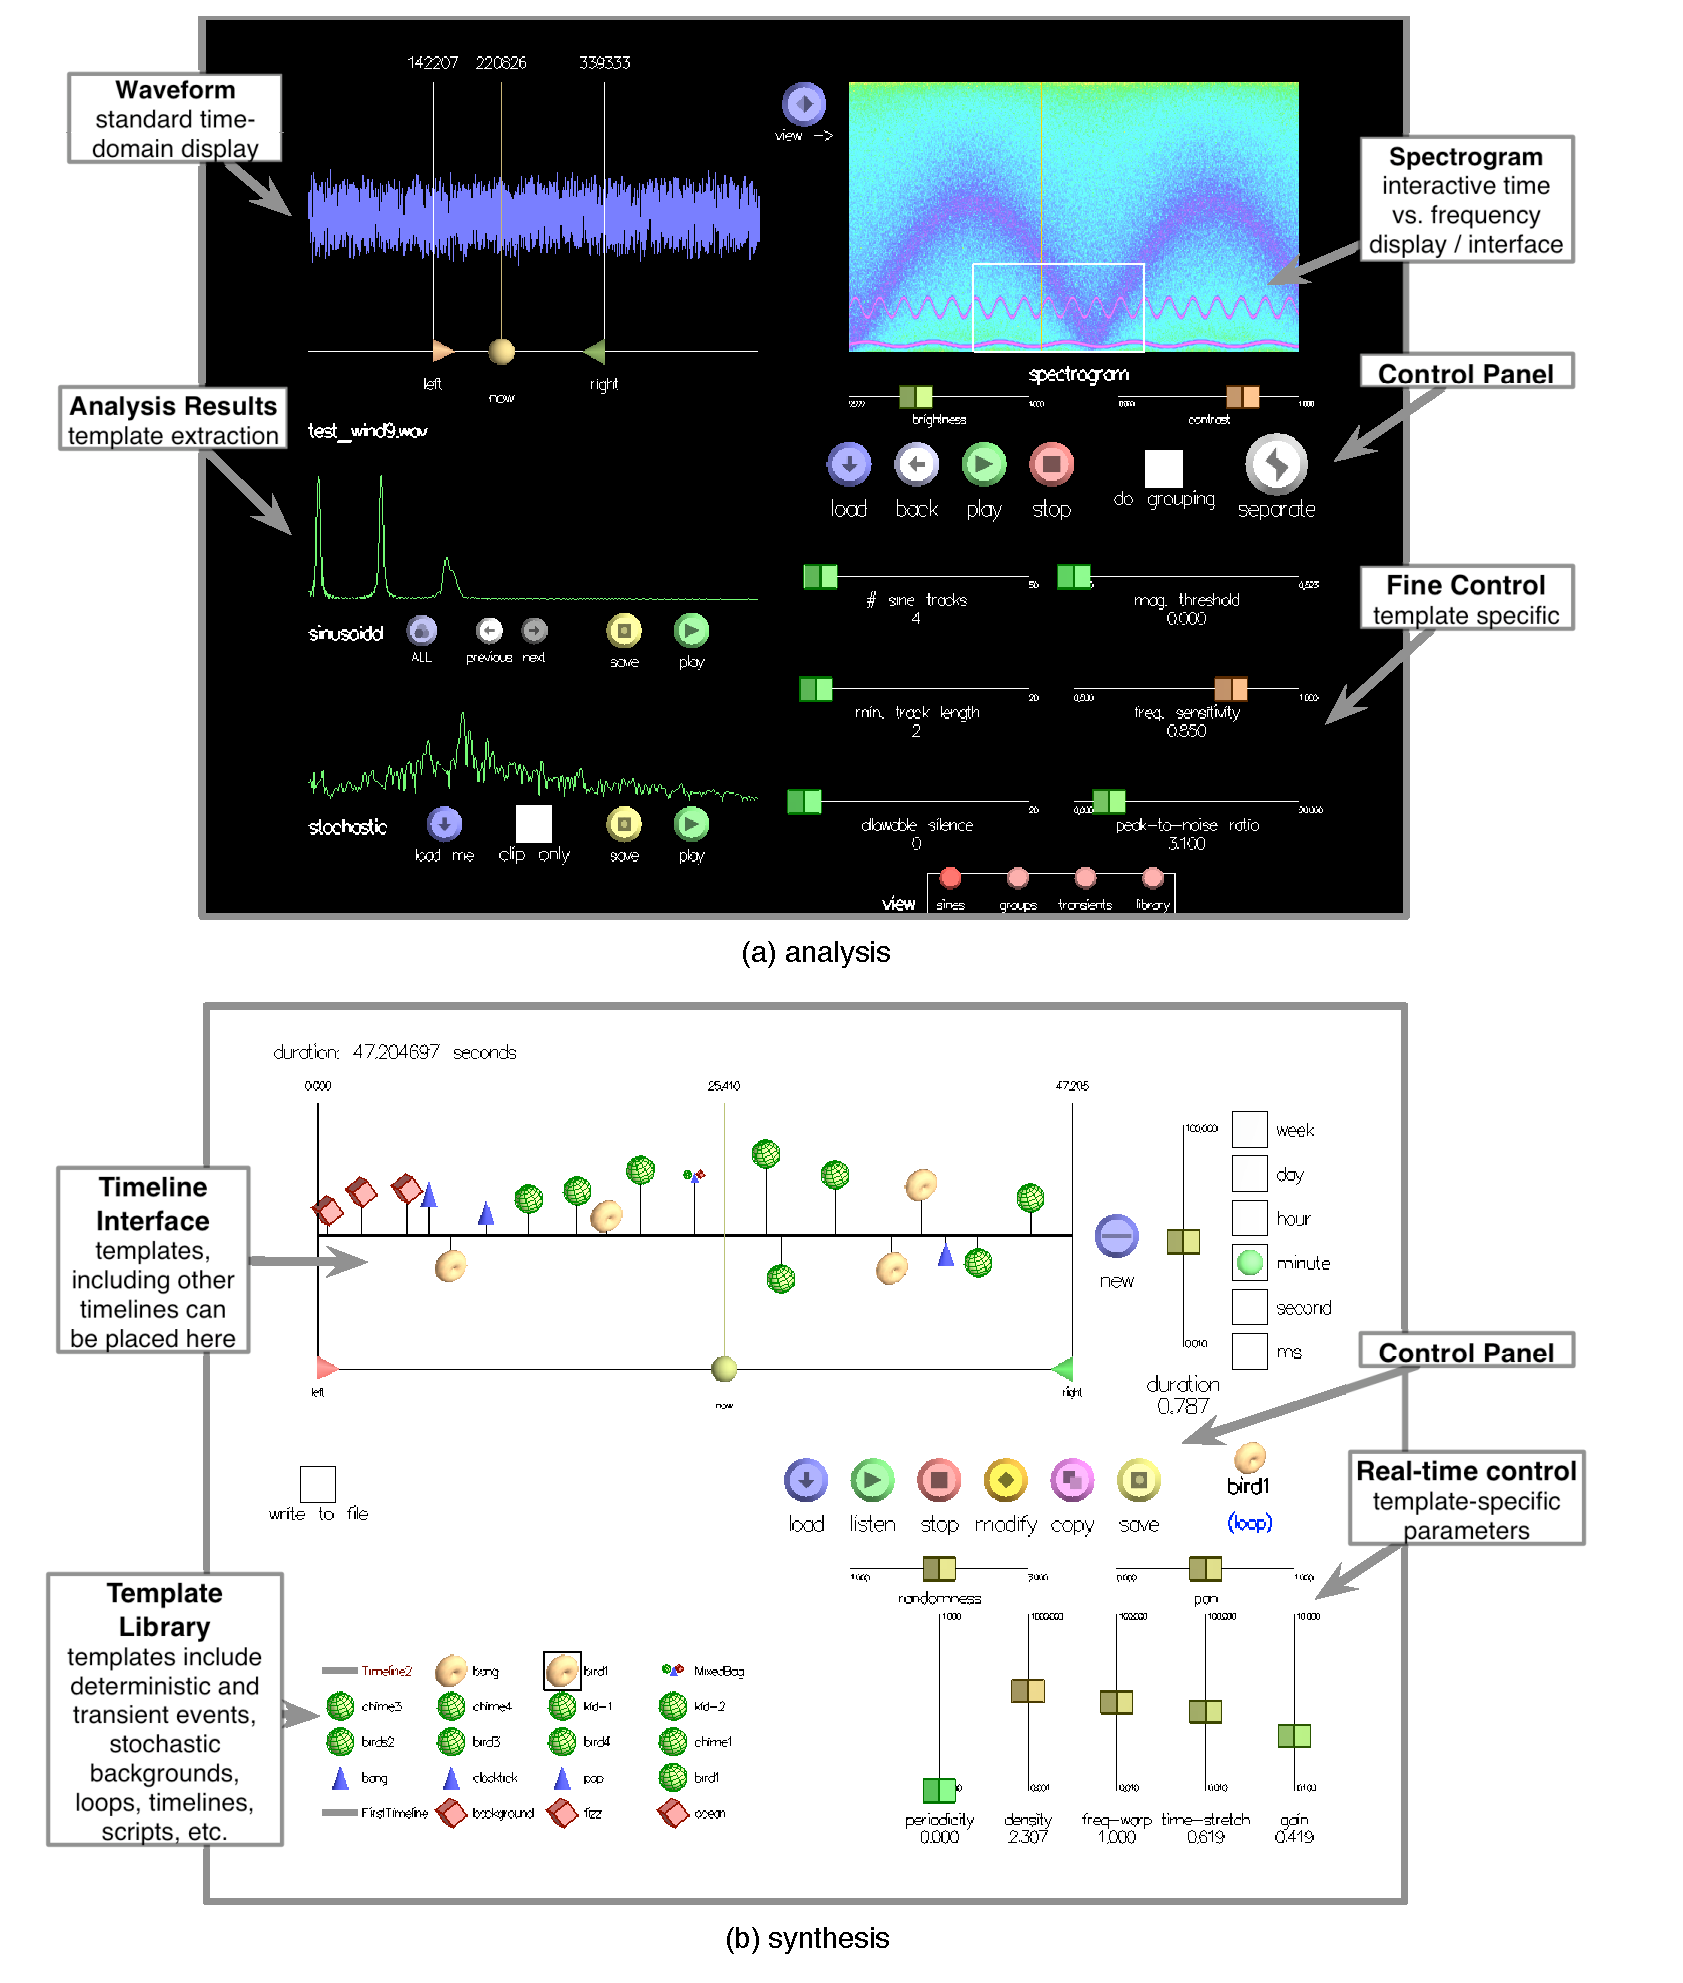
\includegraphics[width=.5\textwidth]{ui2.eps}
%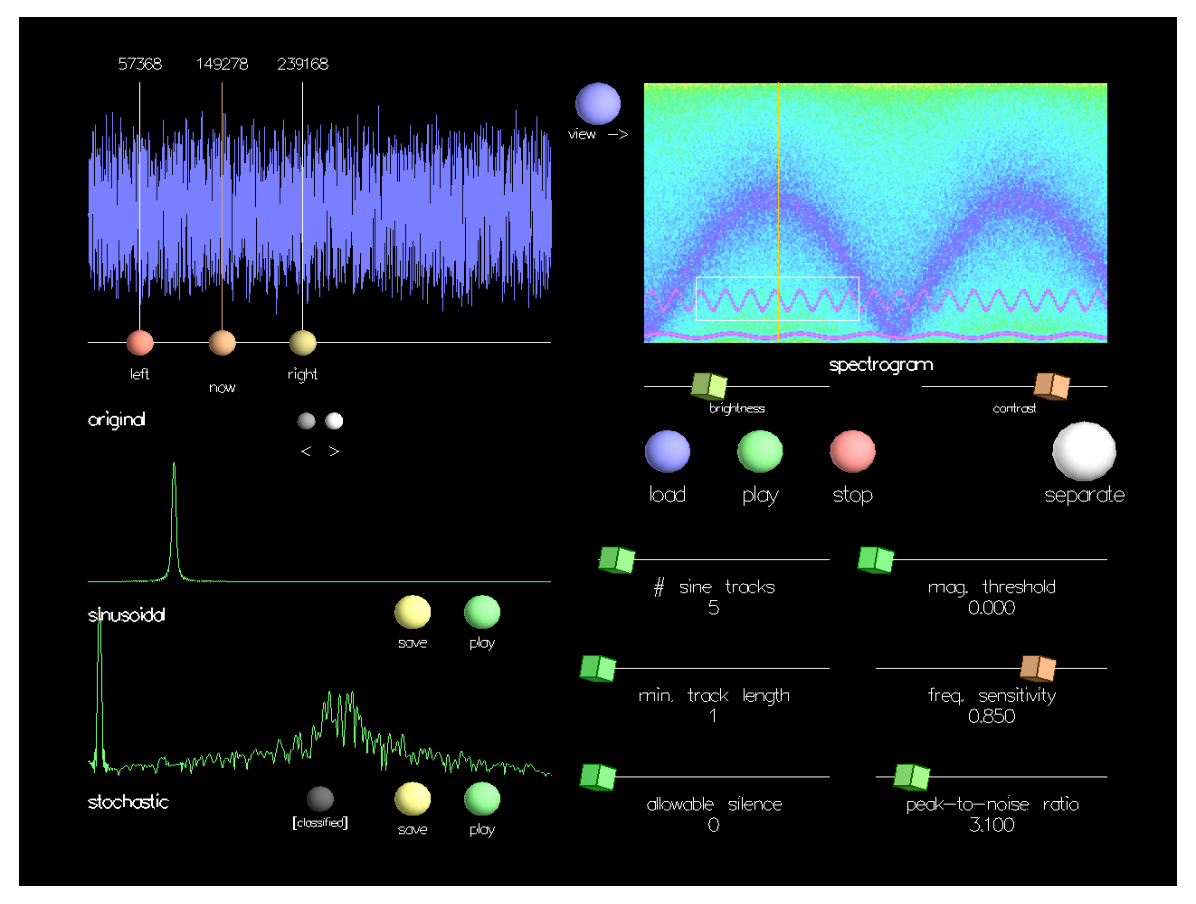
\includegraphics[width=\textwidth]{ui_analysis.eps}
%\subfigure[analysis]{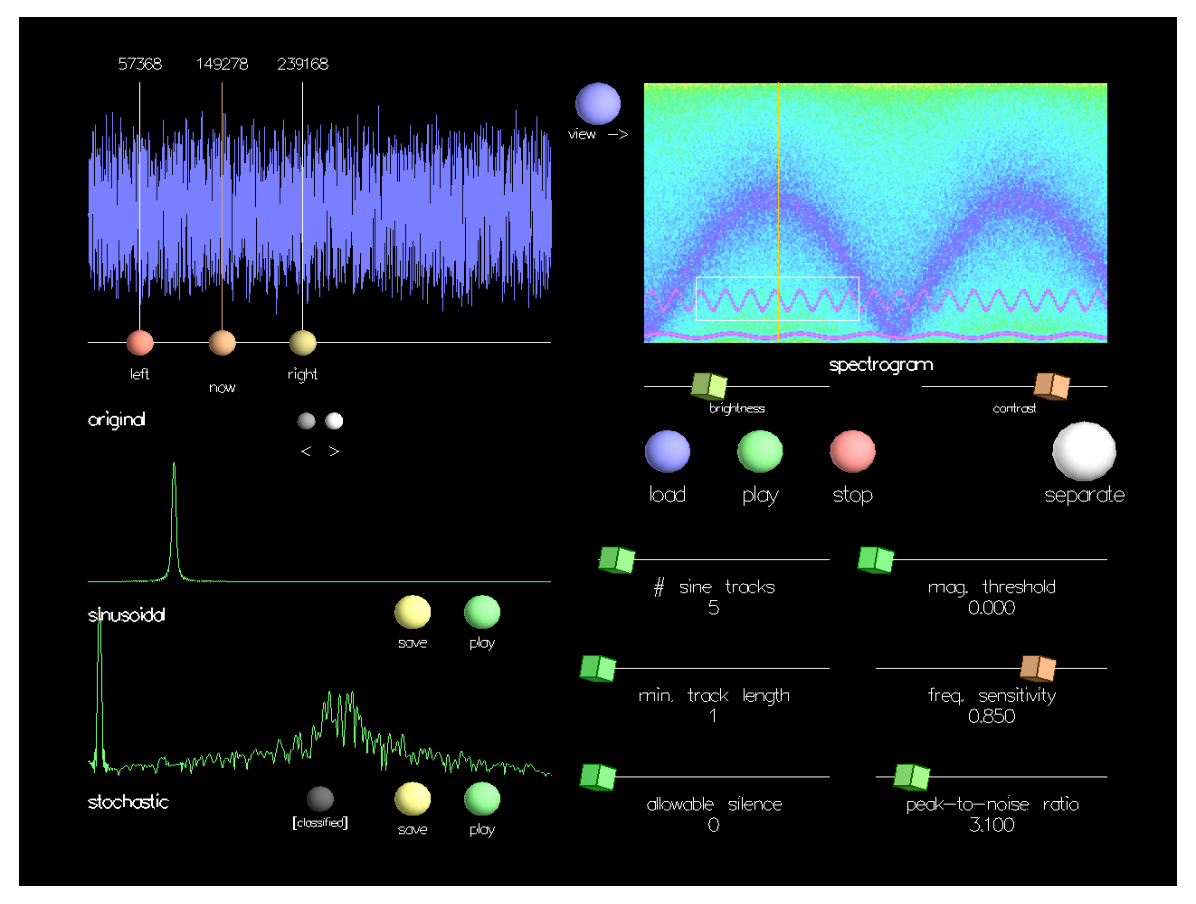
\includegraphics[width=.44\textwidth]{ui_analysis.eps}}
%\subfigure[synthesis]{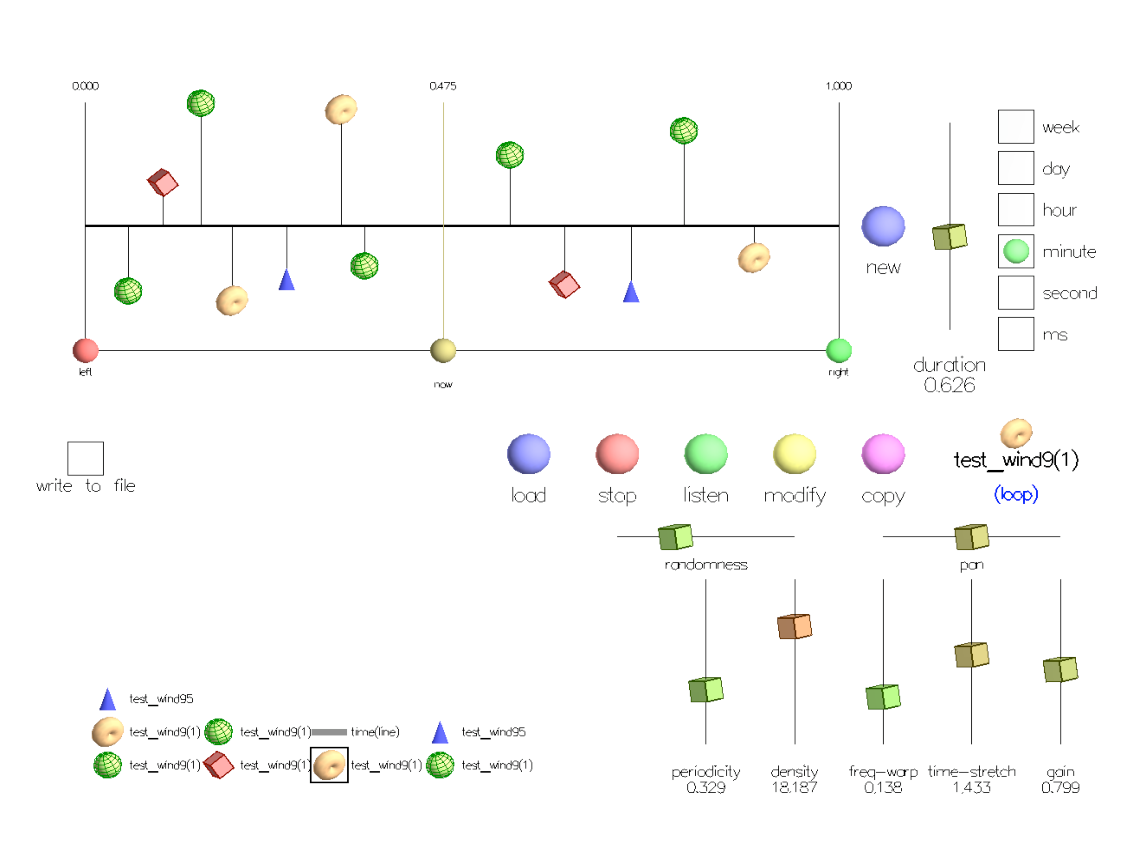
\includegraphics[width=.44\textwidth]{ui_synthesis.eps}}
\caption{Screen shots of user interface. 
%(a) Analysis: Top-left shows time-domain waveform 
%while top-right shows spectrogram. Separated spectra are at bottom-left 
%and analysis parameters at bottom-right. (b) Synthesis: Top half shows a timeline with 
%templates placed on it. Bottom-left shows templates in library; bottom-right shows controls 
%for selected loop template.
} %\clearpage 
\label{fig:ui}
%\end{figure*}
\end{figure}
The synthesis stage of the interface offers a framework for applying 
transformations and synthesizing the resulting sounds. Templates 
saved from the analysis stage are available in the synthesis stage for 
listening, transforming, and placing in a sound scene. Templates 
include the following types: (1) \emph{deterministic events}, (2) \emph{transient events}, (3) 
\emph{stochastic background}, (4) \emph{loops}, and (5) \emph{timelines}. 
The first three are imported directly from the analysis results, while loops 
and timelines are as described in Section 5.1. 
Any event can be saved as a loop, with parameters specifying how often it repeats 
and how periodic the repetition is. Individual event instances within a loop can also be 
randomly transformed within a controllable range, so that every 
iteration of the loop sounds slightly different. This is useful in 
generating `crowd' sounds, such as a flock of birds constructed from a 
single extracted chirp, or many people from a single voice. 
While loops parametrically repeat a single event, timelines control the explicit  
temporal placement of any number of components for a specified duration.  
Any existing template can be dragged on to a timeline; its location on the 
timeline determines when it is synthesized. 
When a timeline is played, each template on it is synthesized at the appropriate 
time step and played for its duration or until the timeline ends. 
It is also possible to place 
timelines within timelines, to capture details of a sound scene at different 
temporal resolutions. Any synthesized sound scene can be written to file while it 
plays, or play forever.  

\section{Results and Contributions}

Figure ~\ref{fig:traffic} shows an example where a single 
existing sound scene is transformed into a different one. 
An original 6 second recording from a warehouse
environment, with some background noise, a multi-toot horn,
and a door slamming was analyzed. The multi-toot horn
was extracted and saved as multi-toot and single-toot deterministic event 
templates. The door-slam transient and final stochastic background sound were separated. 
A new scene of length 19 seconds was constructed using randomized non-looping wavelet
tree re-synthesis for the background. The
new scene combines multiple and overlapping versions
of frequency and time shifted single horns,
a multi-toot horn, and door slams (some transformed
so greatly that they sound like explosions). 
%Sample results can be heard at http://taps.cs.princeton.edu.

\begin{figure}[t]
\centering
\includegraphics[width=.95\columnwidth]{traffic.eps}
\caption{Existing sound scene (top) lengthened and transformed (bottom) with time/frequency 
warps and continuous background}
\label{fig:traffic}
\end{figure}
Our main contributions comprise of the approach and framework for analysis, transformation, 
and synthesis of sound scenes.  In particular, they are (1) techniques and paradigms for 
interactive selection and extraction of templates from a sound scene, (2) techniques for 
parametrically transforming components independently of each other, (3) a 
framework for flexible resynthesis of events and synthesis of novel sound scenes, (4) an 
interface to facilitate each analysis and synthesis task.  Furthermore, we 
have refined several of the core algorithms employed in our system, as follows.

Firstly, we extend the wavelet tree algorithm to 
continually resynthesize the background component, by speeding up the learning. Results show a 4x speedup 
in total running time between the original algorithm (15 levels) and our modified version (stopping 
at 9 levels), for a 1 minute 58 second sound clip to be generated from an 18 second clip sampled at 
11 kHz.

%The results
%\dag 
%in Table 
%\ref{tab:treesynth} were obtained by applying the 
%original and modified wavelet tree learning on a sound clip of length 18 seconds (sample rate 
%11 kHz) to generate 1 minute 58 second sound clips. These show a 4x speedup in 
%total running time between the default algorithm (c) and our modified version (b), even 
%taking into account the additional expense we incur by consulting a growing number of 
%predecessor nodes at each level. The clips synthesized at this additional expense tend to 
%sound more stable.

%\begin{table}[h]
%\begin{center}
%\begin{tabular}{|l|c|c|c|}
%\hline
%  & Learning stop level & Predecessors (k) & Time (sec) \\ \hline
%(a) & 9 & fixed & 1.5 \\
%(b) & 9 & varying & 1.5 \\
%(c) & 15 & fixed & 6 \\
%5(d) & 15 & varying & 12 \\ \hline
%\end{tabular}
%\caption{Wavelet tree learning performance results: 
%Computations took place at error threshold 25\%. The number of predecessors 
%consulted was {\bf fixed} at 5 for all levels, or {\bf varying} as 0.3 times 
%the number of nodes in the level. The original sound decomposed into a {\bf 15-level} 
%wavelet tree; the modified algorithm stopped learning after {\bf level 9}.} 
%\label{tab:treesynth}
%\end{center}
%\end{table}

Secondly, we refine the sinusoidal extraction process by letting users 
parametrically extract specific events. 
%Also, precomputing sinusoidal peaks can 
%yield performance gains of up to 80\% (typical extractions take on the order of milliseconds to seconds). 
The data structures for grouping and storing sinusoidal tracks as 
objects are also a first step towards object classification and 
computational auditory scene analysis \cite{Bregman90}. 

Thirdly, we use wavelet tree learning to fill in the gap left by 
transient removal (Section 4.2). A clear sonic difference
can be discerned between attenuating the transient segment to the noise floor versus 
automatically replacing it with a stochastic sound clip 
produced by wavelet tree learning. 

%On the whole, TAPESTREA simplifies the creation of complex sound scenes from existing ones. 
%without the need for ``untainted'' versions of component sounds. 
%It can extract sound 
%components from complex sounds, synthesize a complete sound scene 
%in real-time with parametric control, leverage 
%parametric sinusoidal modeling to transform deterministic components on a larger scale 
%than other tools, and synthesize unlimited, non-repeating background. 
%Our framework is, to our knowledge, the first to 
%provide a comprehensive approach 
%for extracting/ transforming/ resynthesizing the different component templates, first
%individually, then into cohesive sound scenes.

\section{Conclusion and Future Work}

We have described a framework for extracting specific parts of existing sound scenes and 
flexibly reusing these to create new sound scenes of arbitrary length. 
It allows users to interactively highlight points of interest in the input 
sound, separating it into well-defined components. This allows greater control 
over the synthesized scene, letting elements from different 
sound scenes be transformed independently and combined.
%Unlike existing approaches, our framework separates a given sound into well-defined 
%components, which allows a greater 
%level of control over the variety and quality of the synthesized scene.
We have also demonstrated an interactive paradigm for building new sound scenes, which 
includes iterative refinement of components, interactive previews of transformations, 
grouping, and placement 
in time and space.  Due to the separation, our system is effective in analyzing and 
synthesizing many classes of sounds. It is, to our knowledge, the first to 
provide a comprehensive approach 
for extracting/ transforming/ resynthesizing the different component templates, first
individually, then into cohesive sound scenes.

While our system has no fundamental restriction on the type of input sound to analyze,
%model,
there are some limitations. 
%Our system has some limitations.
When two events overlap in both time and frequency, it can be hard for the
analysis to distinguish between them. Also, when events have strong deterministic as well as 
stochastic components, these components get separated and may be difficult to regroup. 
%Can regroup with a timeline, but what if you want them in a loop? Can timelines be in loops?
%Of course, this can also be viewed as an advantage as it allows components to be 
%mixed in different ways. 
%What about events that have strong deterministic and stochastic 
%components?  What about long time-scale events with complex temporal and spectral behavior?
%Example: like a motorcycle? Also, foreground vocals (such as children singing/yelling) or many 
%musical sounds are difficult to capture faithfully.
Future work includes overcoming these limitations by (1) using more sophisticated event tracking 
and grouping methods, and (2) extending the idea of objects to include composite events with both 
deterministic and transient components. In addition, we plan to combine machine learning techniques 
to classify events and to improve performance without human assistance over time. We would also like to 
extend the precomputing capacities of the system. 

To sum up, our main contributions comprise the approach, system, and interface for 
selective extraction, transformation, and resynthesis of sound scenes. While there is 
plenty of scope for future work, TAPESTREA makes it possible to create novel sound scenes 
from existing sounds in a flexible and parametrically controlled manner, providing a new paradigm 
for both real-time and offline sound production.

\section{Acknowledgements}
Thanks to members of the Princeton soundlab and graphics group. 

%\newpage
\bibliographystyle{IEEEbib}
\bibliography{template} % requires file template.bib

\end{document}
